\section{Results}
 \begin{wrapfigure}{r}{0.45\columnwidth}
\vspace{-5em}
		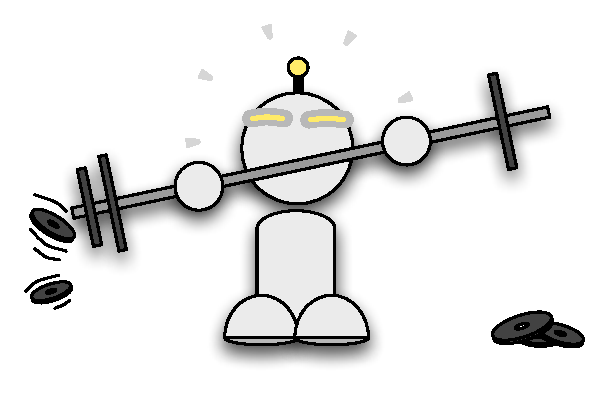
\includegraphics[width=0.45\columnwidth, trim=10mm 0mm 0mm 0mm]{diagrams/robot_weights.pdf}
 \end{wrapfigure}

We evaluate our speedup technique by comparing the performance of A* on a range of realistic and synthetic benchmarks:
\newline 
\textbf{Adaptive Depth} is a set of 12 maps of size 100$\times$100 in which approximately
$\frac{1}{3}$ of each map is divided into adjacent rectangular rooms of
varying size and the rest of the map is a large open area with randomly placed obstacles.
\newline
\textbf{Baldur's Gate} is a set of 120 maps taken from BioWare's popular
roleplaying game \emph{Baldurs Gate II: Shadows of Amn}. 
These maps range in size from 50$\times$50 to 320$\times$320.
\newline
\textbf{Rooms} is a set of 300 maps of size 256$\times$256 which are divided into 32$\times$32
rectangular areas that are connected by randomly placed entrances.
\newline 

A summary of our results is presented in Figure \ref{fig:speedup}.
When searching on our pruned grid maps A* finds optimal length solutions to all problem 
instances 2-4 times faster than otherwise.
A* also explores between 2-3 times fewer locations on average. 
The fastest instances are observed on maps with large open areas.
In such cases we eliminate large numbers of tiles from the interior of each room 
and produce very small grid maps. 
Such an example is shown in Figure \ref{fig:csc2f}.

 \begin{figure}[t]
	\label{fig:csc2f}
	\centering
	\subfigure[A* running on a standard grid map.] {
	%\vspace{-5em}
		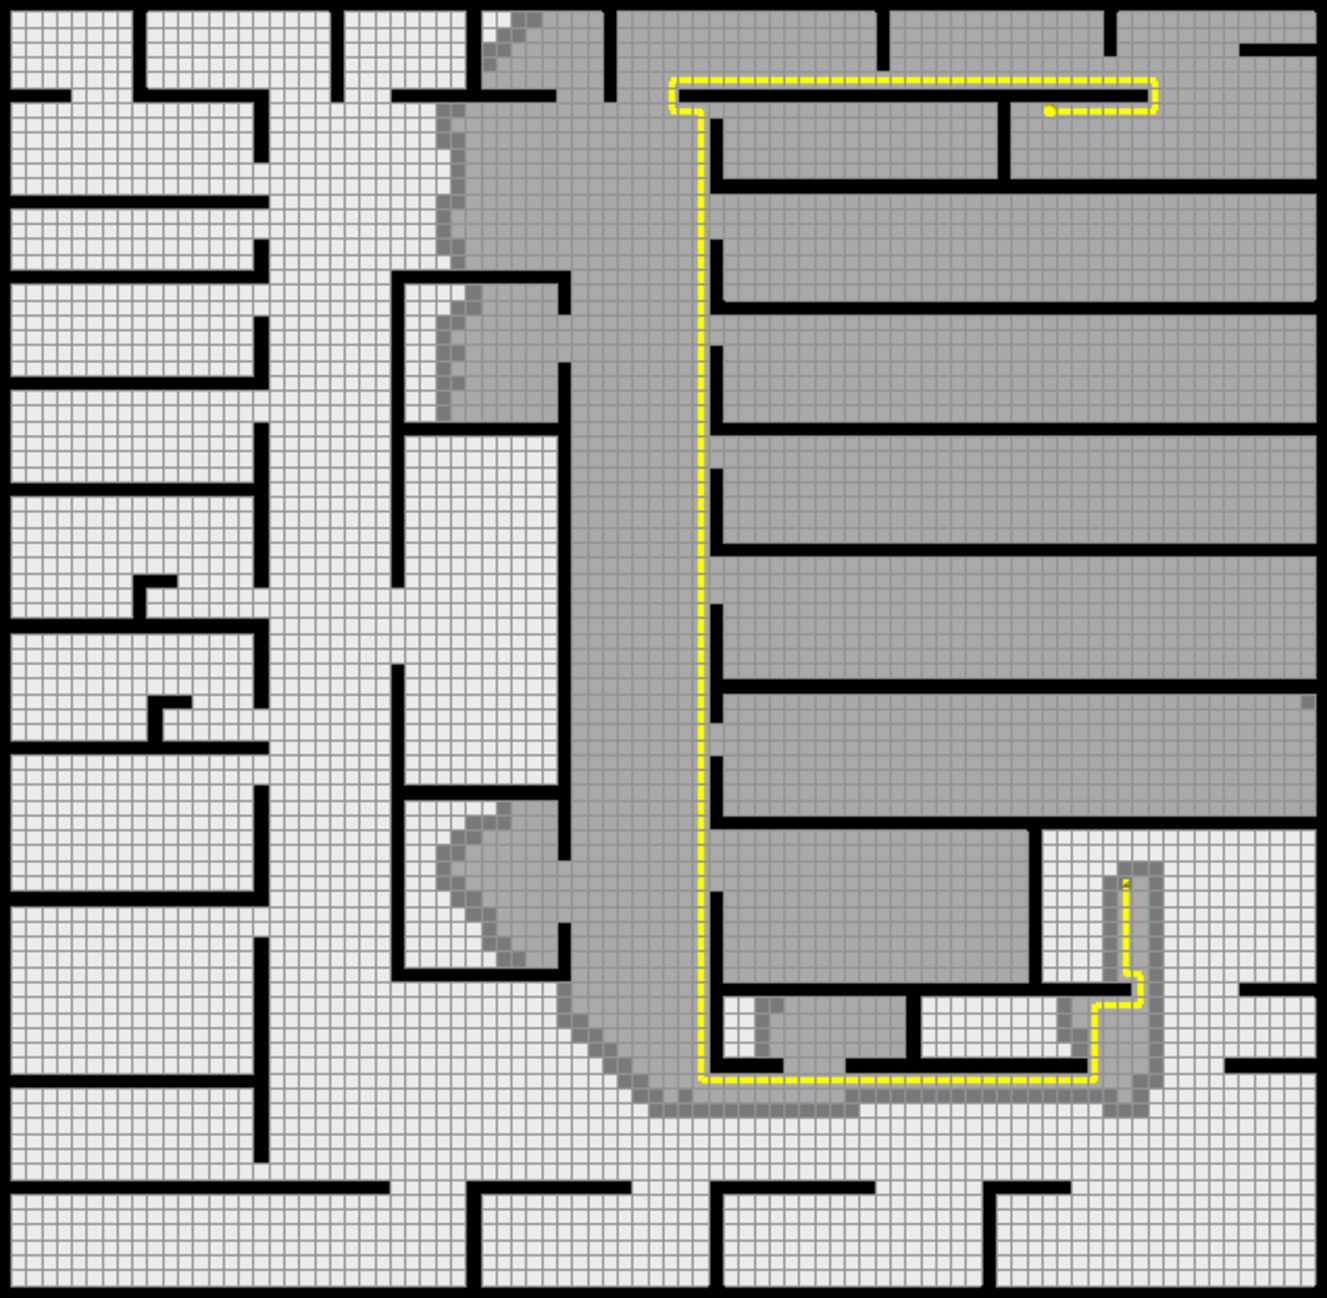
\includegraphics[width=0.47\columnwidth]{diagrams/astarsearch.pdf}
	}
	\subfigure[A* running on our pruned grid map.] {
	%\vspace{-5em}
		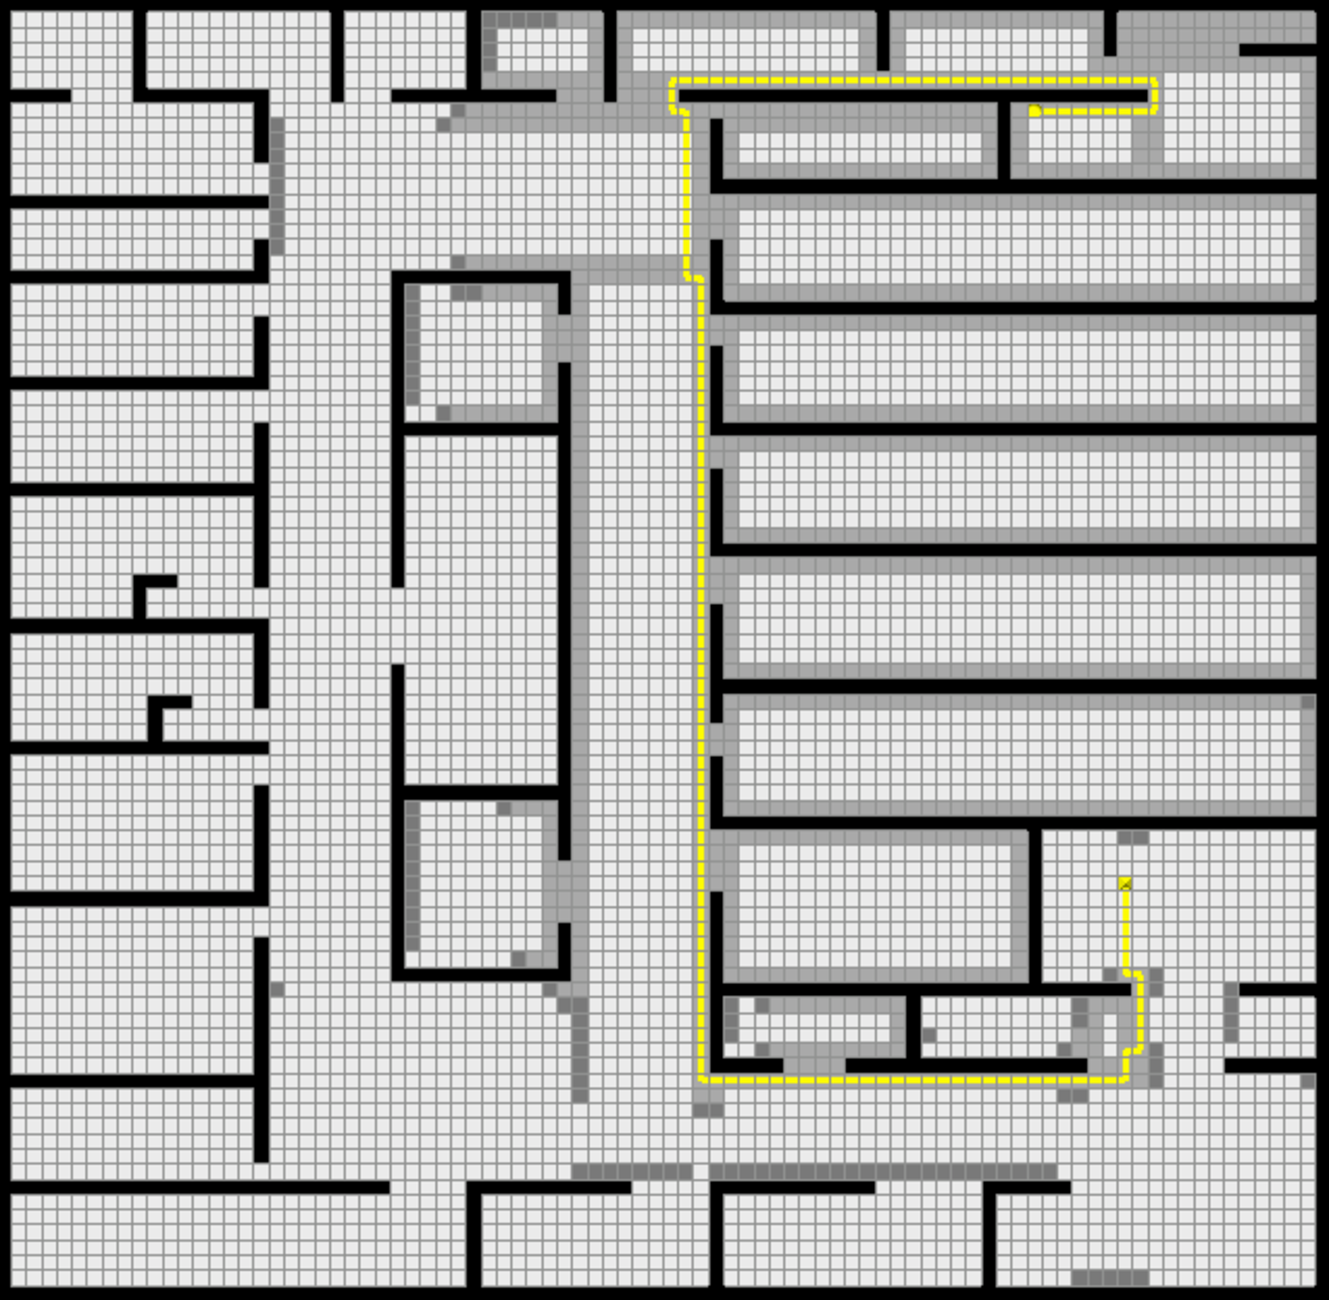
\includegraphics[width=0.47\columnwidth]{diagrams/psearch.pdf}
	}
\caption{Comparative performance of A* on a typical pathfinding problem.
Gray areas are locations which have been explored. 
Using our pruned grid map A* finds the optimal solution 4 times faster}
\vspace{1em}
 \end{figure}
